\section{The Standard Model} \label{sec:theory:standardmodel}

At the turn of the 20th century humanities understanding of the constituent
matter of the universe was limited to what could be seen with microscopes and
implied from the observations of light and electricity, giving evidence for
both the photon and the electron.  In the first half of the century the field
of subatomic physics was discovered with Rutherfords 1911 gold foil scattering
experiment \cite{Rutherford:1911zz}, and the wave-particle duality of with
Compton's scattering experiment in 1923 \cite{PhysRev.21.483}. These were the
first steps towards a Quantum Field Theory representation of nature.  In the
second half of the century experiments delved deeper to discover that the
nucleus contained structure thus extending the SM to include the complex
mechanics of quarks and gluons \cite{Fritzsch:1972jv}.  With the discovery of
the Higgs in 2012, the Standard Model has become even more firmly established
as can be seen in the high level of agreement between theory experiment in
\Cref{fig:xsection_measurements}.

\begin{figure}[!htbp]
  \begin{center}
    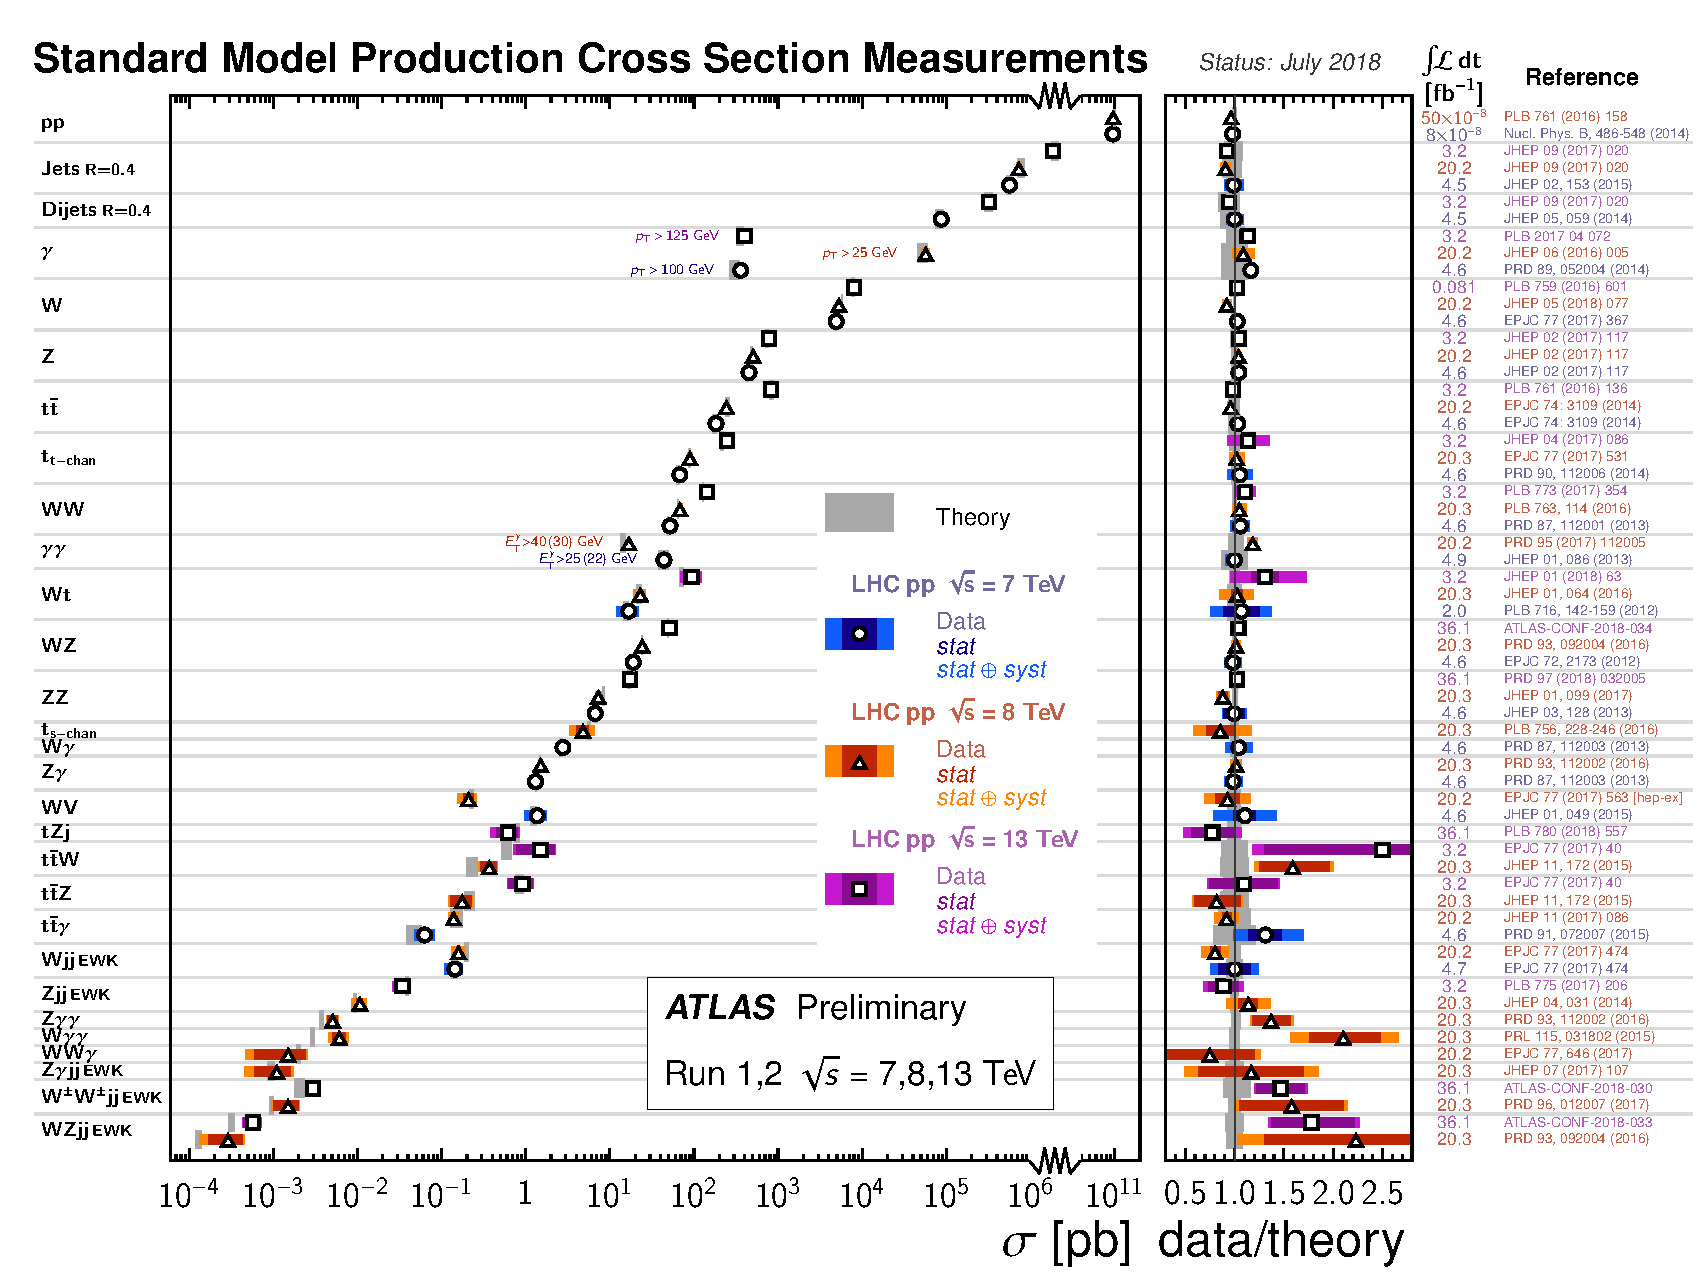
\includegraphics[width=\linewidth]{figures/theory/xsection_measurements.pdf}
\caption{ Summary of several Standard Model total and fiducial production cross
section measurements, corrected for leptonic branching fractions, compared to
the corresponding theoretical expectations \cite{StandardModelPublicResults}.
All theoretical expectations were calculated at NLO or higher. The dark-color
error bar represents the statistical uncertainty. The lighter-color error bar
represents the full uncertainty, including systematics and luminosity
uncertainties. The data/theory ratio, luminosity used and reference for each
measurement are also shown. Uncertainties for the theoretical predictions are
quoted from the original ATLAS papers. They were not always evaluated using the
same prescriptions for PDFs and scales.}
    \label{fig:xsection_measurements}
  \end{center}
\end{figure}

The QCD and GSW theories predict two classes of particles - fermions and bosons -
shown in \Cref{fig:standard_model}. These particles represent the quanta
of the quantum fields of the Standard Model and the mediators of the fundamental
forces of Nature.

\begin{figure}[!htbp]
  \begin{center}
    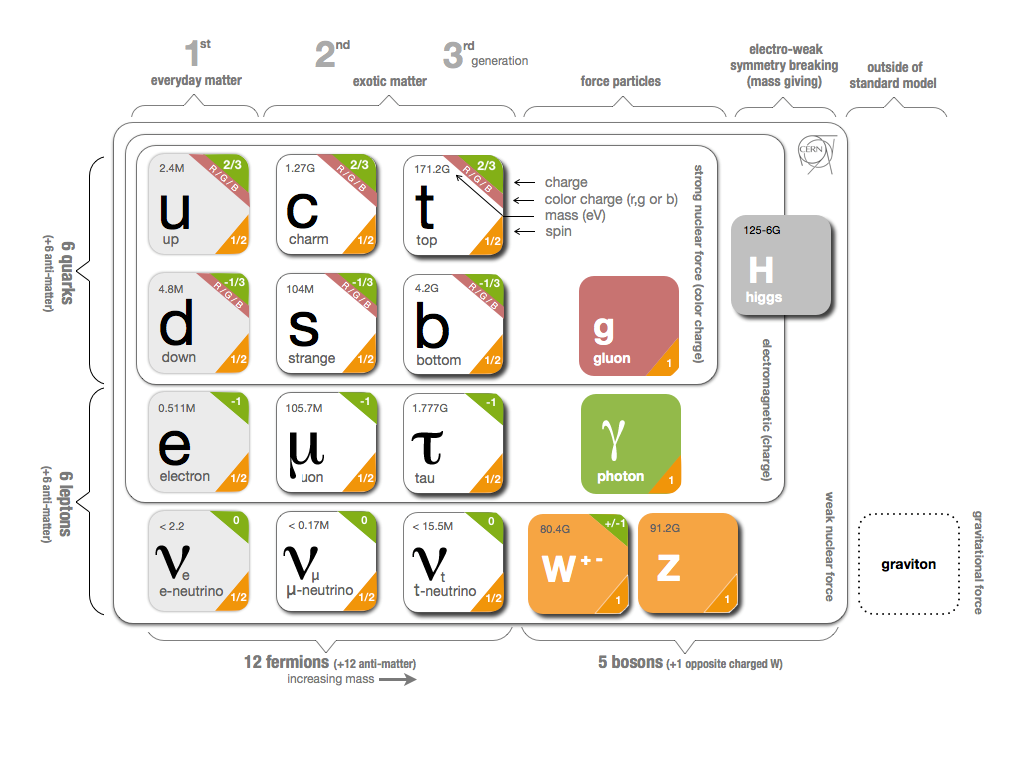
\includegraphics[width=\linewidth]{figures/theory/standard_model.png}
    \caption{ Table of all observed fundamental particles of the Standard
Model. \cite{Purcell:1473657}}
    \label{fig:standard_model}
  \end{center}
\end{figure}

\subsection{Bosons} \label{sec:theory:bosons}

The spin-1 particles are known as the vector gauge bosons and are the force
carriers of the SM.  The most commonly known is the electromagnetic force's
uncharged and massless photon ($\gamma$) which interacts with all charged
particles and is often referred to as ``light."  The weak nuclear force is
involved in nuclear interactions such as beta decays and is carried by 3
bosons, all of which have mass and couple to fermions.  The $W^{\pm}$ bosons
mediate the charged weak interaction and allow for flavor changing currents,
while the $Z$ boson mediates the neutral weak interaction.  Finally there are 8
massless gluons which mediate the strong force and only interact with fermions
that have a ``color" charge such as the quarks contained inside the nucleons. The
only spin-0 boson, the Higgs Boson ($H$) is the key to generating mass terms in
the SM Lagrangian for the massive gauge bosons and for fermions.  This is done
through the so-called Higgs mechanism \cite{Thomson:2013zua} and is discussed
in more detail in \Cref{sec:theory:higgs}.

\subsection{Fermions} \label{sec:theory:fermions}

The spin-1/2 particles can be further broken up into two distinct families of
particles, the leptons and the quarks, both of which contain three
``generations" each with an ``up"- and ``down"-type particle where ``up" and
``down" differentiate the two components of the weak isospin doublet.  The
``down"-type leptons are the electrically charged electron ($e$), muon ($\mu$)
and tau ($\tau$) while the ``up"-type are their electrically neutral
counterparts $\nu_e$, $\nu_\mu$, $\nu_\tau$. The ``up"-type quarks are the up
($u$), charm ($c$), and top ($t$), each with a $+2/3$ electric charge, while
the ``down"-type quarks are the down ($d$), strange ($s$), and bottom ($b$),
all of which have a $-1/3$ electric charge.  Each quark carries a ``color"
charge thus allowing them to couple to gluons and  participate in strong force
interactions.  Due to the observed color confinement of the strong force these
quarks are only observed in colorless bound states known as ``mesons" (1 quark
and 1 anti-quark) and ``baryons" (3 quarks or anti-quarks).  All of the above
fermions have an anti-particle partner with the opposite weak isospin.
